%undeveloped code: RNN, sys, bo

\documentclass{beamer}
%\usepackage{cite} %\bibliographystyle{IEEEtran}
\usepackage{pgfpages}
\usepackage[backend=bibtex,style=authortitle-ibid]{biblatex}
\bibliography{IEEEfull,library}
\usepackage{xcolor}
\usepackage{array} \usepackage{makecell}
\usepackage{colortbl}

%\addbibresource{library.bib}
\usetheme{metropolis}           % Use metropolis theme
\title{Unsupervised Anomaly Detection in Sequences
Using Long Short Term Memory Recurrent Neural Networks}
\date{April 20, 2016} %
\author{Majid S. alDosari}
\institute{George Mason University}


\setbeameroption{show notes}% on second screen=left}

\AtBeginSubsection{\frame{\subsectionpage}}

\usepackage{amsmath,amssymb}
%matrix
\newcommand{\mt}[1]{\ensuremath{\mathbf{#1}}}
%vector
\newcommand{\vc}[1]{\ensuremath{\boldsymbol{#1}}}
%set
\newcommand{\st}[1]{\ensuremath{\mathcal{#1}}}
%time index
\newcommand{\tm}[1]{\ensuremath{\sp{(#1)}}}


%x
\newcommand{\x}[0]{\ensuremath{\vc{x}}}
%s
\newcommand{\s}[0]{\ensuremath{\vc{s}}}
%W
\newcommand{\W}[0]{\ensuremath{\mt{W}}}


\begin{document}

  \maketitle

  \begin{frame}[allowframebreaks]{Contents}
    \tableofcontents 
  \end{frame}

  \section{Introduction}

  \begin{frame}{Modern technology facilitates the 
      capture, storage, and processing of sequential data at scale}

    \begin{itemize}
    \item Data capture
      \begin{itemize}
      \item physiological signals
      \item network traffic
      \item industrial processes
      \item automobiles
      \item website navigation
      \item environment
      \end{itemize}
    \item Data storage
      \begin{itemize}
      \item Hadoop
      \item MongoDB
      \end{itemize}
    \item Ubiquitous computing
      \begin{itemize}
      \item cloud/cluster
      \item desktop
      \item at point of capture
      \end{itemize}
    \end{itemize}    


  \end{frame}


  \begin{frame}{Problem: Finding anomalous data is challenging}

    \begin{itemize}
    \item large 
    \item varied
    \item domain knowledge required
    \end{itemize}

  \end{frame}


  \begin{frame}{Solution: Use recurrent neural networks to generically find anomalous data}

    \begin{itemize}
      \item This work:
    \begin{enumerate}
      \item Background: Anomaly detection in sequences
      \item Sequence Modeler: Recurent neural network (RNN)
      \item Experiments: RNNs for anomaly detection
    \end{enumerate}

    \item Prior: Malhotra \footcite{Malhotra2015} but no emphasis on process
    \note{i actually had a discussion with him}
    \end{itemize}

  \end{frame}


  \section{The Challenge of Anomaly Detection in Sequences}

  \begin{frame}{Anomaly dectection work is fragmented}
    \begin{itemize}
    \item variety of solutions in communication networks, biology, economics, biology, ...etc.
    \item different settings
    \item no comparison between application domains
    \item technical basis in computer science vs. statistics
    \item not much review literature:
      Cheboli\footcite{Cheboli2010}
      and Gupta\footcite{Gupta2013}
    \end{itemize}
  \end{frame}


  \begin{frame}{Define the problem to focus on the right solution}

    Sequence $\x$
    \begin{gather*}
      \x=\{\x\tm{1},\x\tm{2},\x\tm{t},\ldots,\x\tm{T}\} \\
      \x\tm{t} \in \mathbb{R}^v
    \end{gather*}%

    Assumption: Anomalies are a small part of the data.

  \end{frame}


  \begin{frame}{Solution must answer the following:}

    \begin{enumerate}
    \item
      \textcolor{red}{What is normal (as an anomaly is defined as what is \textit{not} normal)?}
    \item
      What measure is used to indicate how anomalous point(s) are?
    \item
      How is the measure tested to decide if it is anomalous?
    \end{enumerate}

  \end{frame}


  \begin{frame}[allowframebreaks]{Solution must address different anomaly types}

    Simple point anomaly
    \centering
    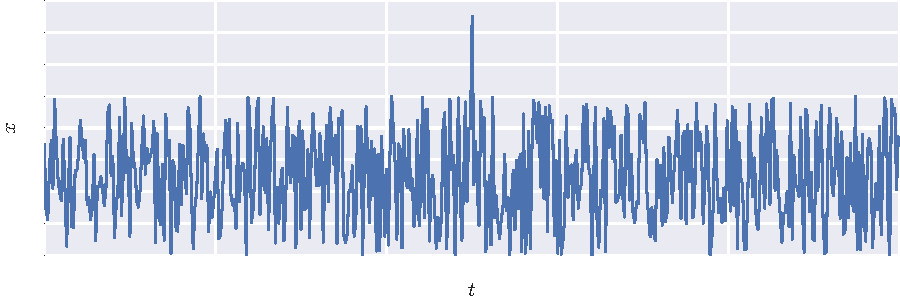
\includegraphics[width=\textwidth]{figs/trivial.pdf}

    \framebreak
    Anomaly in a periodic context
    \centering
    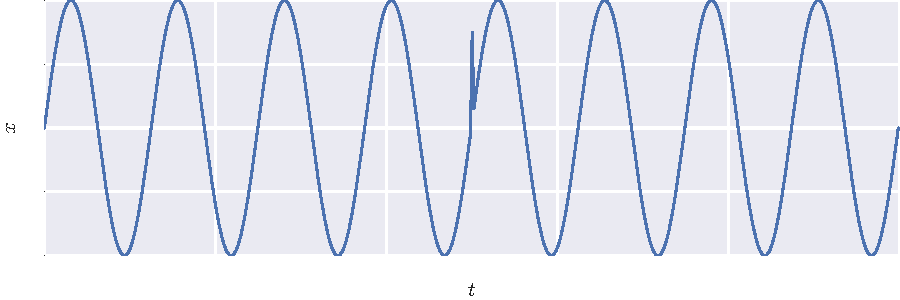
\includegraphics[width=\textwidth]{figs/context.pdf}

    \framebreak
    Discord anomaly in a periodic time series
    \centering
    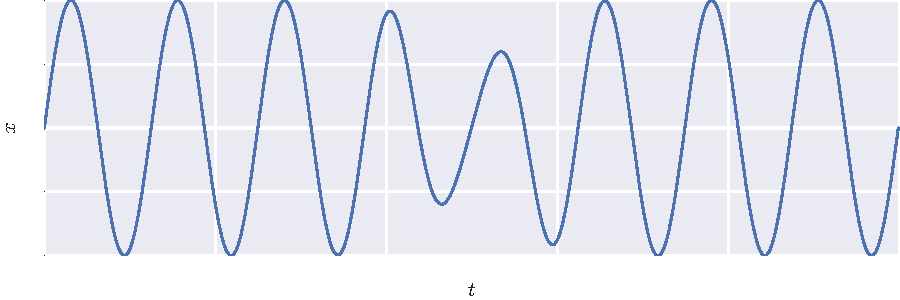
\includegraphics[width=\textwidth]{figs/discord_per.pdf}

    \framebreak
    Discord anomaly in an aperiodic time series
    \centering
    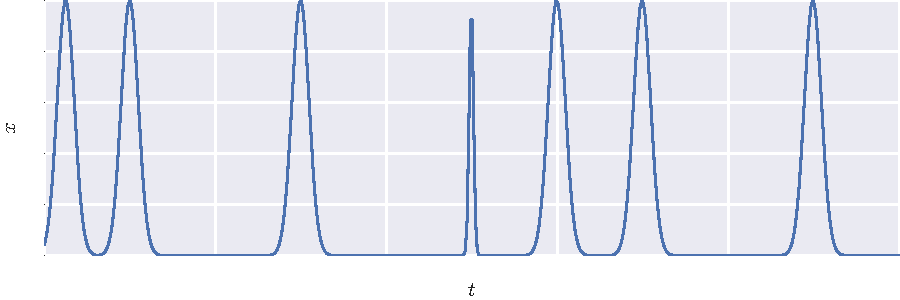
\includegraphics[width=\textwidth]{figs/discord_aper.pdf}

    \framebreak
    \centering
    Multivariate: (a)synchronous and (a)periodic

  \end{frame}


  \section{Procedure}

  \begin{frame}{Description of anomaly detection procedure is straightforward}

    \begin{enumerate}
    \item Compute an anomaly score for an observation
    \item Aggregate the anomaly scores for many observations.
    \item Use the anomaly scores to determine whether an observation can be considered anomalous
    \end{enumerate}

  \end{frame}

  \begin{frame}{Characterizing normal behavior is involved}
    
    \begin{equation*}
    \x=\{\x\tm{1},\x\tm{2},\x\tm{t},\ldots,\x\tm{T}\}
    \end{equation*}

    \begin{enumerate}
    \item Extract Samples
    \item Transform Samples
    \item Apply Detection Technique
    \end{enumerate}

  \end{frame}


  \subsection{1. Sample Extraction}
  
  \begin{frame}{Use sliding windows to obtain samples}
    
    \begin{center}
    $\mathcal{X}=\{W_1,W_2,\ldots,W_p\}$
    \end{center}

    \begin{itemize}
      \item hop, $h$
      \item window, $w$ %for localizing anom
    \end{itemize}

  \end{frame}


  \begin{frame}{Problem: Hops can skip over anomalies}

    \begin{center} 
     sequence: \emph{abc\underline{c}abcabc} 

      \begin{tabular}{|c|c|}
        \hline
        hop ($h$) & Ordered Windows \\
        \hline
        \hline
        1 & \emph{abc},
            \emph{bc\underline{c}}, 
            \emph{c\underline{c}a}, 
            \emph{cab},
            \emph{abc}, 
            \emph{bca},
            \emph{cab},
            \emph{abc} \\
        \hline
        2 & \emph{abc},
            \emph{c\underline{c}a},
            \emph{abc},
            \emph{cab} \\
        \hline
        3 & \emph{abc}, 
            \emph{cab},
            \emph{cab} \\
        \hline
        4 & \emph{abc}, 
            \emph{abc} \\
        \hline
      \end{tabular}

    \end{center}
    
  \end{frame}


  \begin{frame}{Problem: Window size must be large enough to contain anomaly}

    \begin{center}
      sequence:
      \emph{aaabbbccc\underline{c}aaabbbcccaaabbbccc}
    \end{center}

    Window width must be at least 4.

  \end{frame}


  \begin{frame}{Problem: Treating window width as a dimension ignores temporal nature}

    \begin{gather*}
      \mathcal{X} =\{W_1,W_2,\ldots,W_p\}   \\
      W \in \mathcal{R}^{1 \times w}
    \end{gather*}
    
  \end{frame}


  % \begin{frame}{Problem: Windows and hop size can't be too lage}

  %   \begin{center}
  %     sequence:
  %     \emph{aaabbbccc\underline{c}aaabbbcccaaabbbccc}
  %   \end{center}

  % \end{frame}


  \subsection{2. Transformation}


  \begin{frame}{Transformation can help reveal anomalies}

    \begin{itemize}
    \item Haar transform %but only if 
    \item Symbolic Aggregate approXimation (SAX) \footcite{Lin2007}
    \end{itemize}

  \end{frame}

  \begin{frame}{Transformation is not general}

    \begin{itemize}
    \item Choice of representation must be compatible with data characteristics  %can't encode pt anom in freq
    \item normal:anomaly as transform(normal):transform(anomaly)
    \end{itemize}

    Study \footcite{Wang2013} suggests generally little difference among representations.

  \end{frame}


  \subsection{3. Detection Technique}

  \begin{frame}{Anomaly detection techniques and their application domains are varied}

    Based on
    \begin{itemize}
    \item Segmentation
    \item Information Theory
    \item Proximity 
    \item Modeling
    \end{itemize}

  \end{frame}

  \begin{frame}{Model and proximity-based techniques are most developed}

    Based on
    \begin{itemize}
    \item Segmentation: requires homogeneous segments
    \item Information Theory: requires finding sensitive information-theoretic measure
    \item Proximity
    \item Modeling
    \end{itemize}

  \end{frame}


  \section{Proximity}


  \begin{frame}{Idealization never occurs}

      \centering
      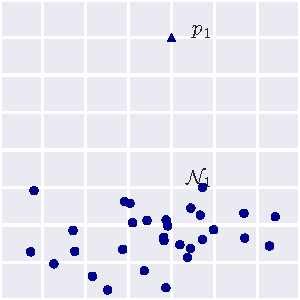
\includegraphics[height=\textheight]{figs/simple_dist.pdf}

  \end{frame}

  \begin{frame}{Practically, distributions are complicated}
    
    \centering
    \begin{tabular}{c|c}
    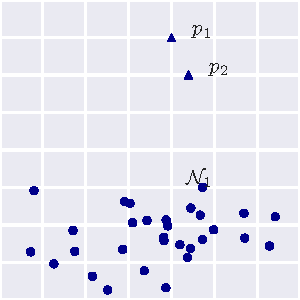
\includegraphics[width=.45\textwidth]{figs/hard1_dist.pdf} &
    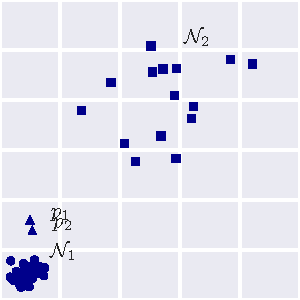
\includegraphics[width=.45\textwidth]{figs/hard2_dist.pdf}
    \end{tabular}

  \end{frame}


  \subsection{Effects on Point Distribution}


  \begin{frame}{Distance measure should be invariant to:}

    \begin{itemize}
      \item length
      \item translation
      \item (skew)
      \item (amplitude)
    \end{itemize}

    Study \footcite{Wang2013}: Not much difference in similarity measures

  \end{frame}

  \begin{frame}{Window width needs to be chosen on the scale of expected anomaly}
    
    % so you might thing oh just make it big
    If width is too large:
    \begin{itemize}
      \item anomalous points not distinguished
      \item data becomes equidistant in high-dimensional space
    \end{itemize}

  \end{frame}


  \begin{frame}{Sliding windows challenge anomaly detection assumptions}
    
    \begin{itemize}
      \item anomalous points are not necessarily in sparce space while repeated patterns are not necessarily  in dense space \footcite{Keogh2005}
      \item ``Clustering of Time Series Subsequences is Meaningless'' \footcite{Keogh2004}
    \end{itemize}

  \end{frame}


  \subsection{Data Classification}

  \begin{frame}{Global vs Local: Local techniques use neigborhood data}
    
    \centering
    \begin{tabular}{c|c}
      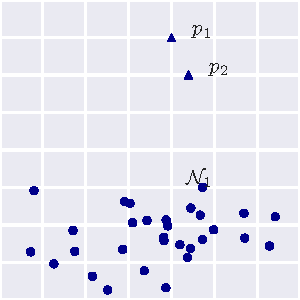
\includegraphics[width=.45\textwidth]{figs/hard1_dist.pdf} &
      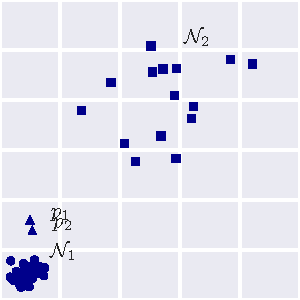
\includegraphics[width=.45\textwidth]{figs/hard2_dist.pdf}
    \end{tabular}

  \end{frame}


  \subsection{Nearest Neighbor}


  \begin{frame}{Overlapping windows distort data similarity}

    \begin{tabular}{lc}
      \emph{abcabcXXXabcababc} &
      \begin{small} 
 %       \begin{center}
          \begin{tabular}{|c||c|}
            \hline
            $h=1$ & $h=3$ \\
            \hline
            \hline
            \emph{abc} & \emph{abc} \\
            \emph{bca} & \\
            \emph{cab} & \\
            \hline
            \emph{abc} & \emph{abc} \\
            \emph{bcX} & \\
            \emph{cXX} & \\
            \hline
            \emph{XXX} & \emph{XXX} \\
            \emph{XXa} & \\
            \emph{Xab} & \\
            \hline
            \emph{abc} & \emph{abc} \\
            \emph{bca} & \\
            \emph{cab} & \\
            \hline
            \emph{aba} & \emph{aba} \\ 
            \emph{bab} & \\
            \emph{abc} & \\
            \hline
          \end{tabular}
%        \end{center}
      \end{small}
    \end{tabular}

  \end{frame}


  \begin{frame}{Solution: Use non-self matches \footcite{Keogh2005}}

    \small
    \centering
    \begin{tabular}{|c||c|}
      \hline
      $h=1$ & $h=3$ \\
      \hline
      \hline
      \emph{abc} & \emph{abc} \\
      \emph{bca} & \\
      \emph{cab} & \\
      \hline
      \emph{abc} & \emph{abc} \\
      \emph{bcX} & \\
      \emph{cXX} & \\
      \hline
      \emph{XXX} & \emph{XXX} \\
      \emph{XXa} & \\
      \emph{Xab} & \\
      \hline
      \emph{abc} & \emph{abc} \\
      \emph{bca} & \\
      \emph{cab} & \\
      \hline
      \emph{aba} & \emph{aba} \\ 
      \emph{bab} & \\
      \emph{abc} & \\
      \hline
    \end{tabular}

  \end{frame}


  \begin{frame}{kNN uses no local information}
    \note[item]{if you can mitigate time series issues}
    \note[item]{ hotsax k=1, go thru 2,3,*4*,5,6 .N2 different density}
    
    \centering
    \begin{tabular}{c|c}
      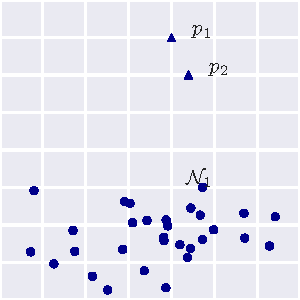
\includegraphics[width=.45\textwidth]{figs/hard1_dist.pdf} &
      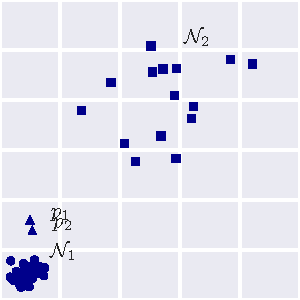
\includegraphics[width=.45\textwidth]{figs/hard2_dist.pdf}
    \end{tabular}

  \end{frame}


  \begin{frame}{Local Outlier Factor\footcite{Breunig1999} uses local density information}
    
    A point is likely to be an anomaly if its neighbors are in dense regions while it is in a less dense region
    \centering
    \begin{tabular}{c|c}
    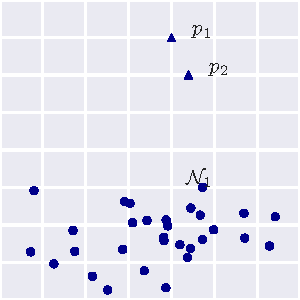
\includegraphics[width=.45\textwidth]{figs/hard1_dist.pdf} &
    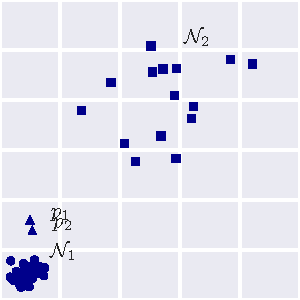
\includegraphics[width=.45\textwidth]{figs/hard2_dist.pdf}
    \end{tabular}
    (Didn't you say anomalies may not be in less dense regions?!)
    
  \end{frame}


  \subsection{Clustering}

  \begin{frame}{Clustering algorithms are usually not designed to find anomalies}

    Assumptions: anomalous points
    \begin{itemize}
    \item do not belong to a cluster (DBSCAN\footcite{Ester1996})
    \item are far from a cluster centroid %see the problem?
    \item are in less dense clusters
    \end{itemize}

  \end{frame}


  \section{Models}

  \begin{frame}{Hidden Markov Models (HMMs) are general advanced sequence modelers}
    
    Restrictions:
    \begin{itemize}
      \item fixed length sequences
      \item Markovian process
    \end{itemize}

  \end{frame}


  \section{Problems with Established Techniques}


  \begin{frame}{How to determine \emph{a priori} what the best algorithm is?}
    
    review papers only give subjective assessments

  \end{frame}


  \begin{frame}{Proximity-based techniques need alot of decisions}
    
    Choose:
    \begin{itemize}
      \item similarity measure
      \item sliding window size
      \item sliding window hop
      \item compatible classification technique
    \end{itemize}

  \end{frame}


  \begin{frame}{Solution: Use a model-based technique}
    
    \begin{itemize}
      \item characterize normal %more elegant. compare with clustering/NN
      \item restriction: use when data \emph{can} be modeled
    \end{itemize}

    Ideally:
    \begin{itemize}
      \item model arbitrary time series
      \item minimize effect of window length
      \item requires as few parameters as possible
    \end{itemize}

  \end{frame}





  \section{Recurrent Neural Networks (RNNs)}

  
  \begin{frame}{RNNs are powerful}
    
    \begin{itemize}

    \item speech recognition
    \item handwriting recognition
    \item music generation
    \item text generation
    \item handwriting generation
      %lstm
    \item translation
    \item identifying non-verbal cues from speech
    \item image caption generation
    \item video to text description
    \item generating talking heads

    \end{itemize}
        
  \end{frame}


  \begin{frame}{RNNs are more flexible and efficient than HMMs}
    
    state:
    \begin{itemize}
    \item HMM: hidden state depends only on previous state
    \item RNN: shared state
    \end{itemize}

    generality:
    \begin{itemize}
    \item HMM: Markovian
    \item RNN: general computation device
    \end{itemize}
    
  \end{frame}


  \begin{frame}{Recurrence explains the efficiency of RNN encoding}
    
    \newsavebox{\recurrent}
\savebox{\recurrent}{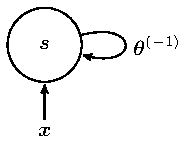
\includegraphics[]{figs/recurrent.pdf}}
\newsavebox{\recurrentuf}
\savebox{\recurrentuf}{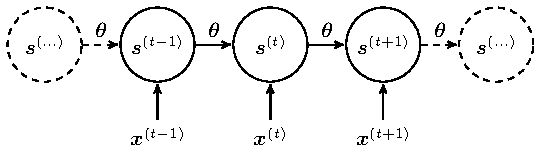
\includegraphics[]{figs/recurrent_uf.pdf}}

cyclic view
    \begin{center} \usebox{\recurrent} \end{center}

acyclic view
    \begin{center}  \usebox{\recurrentuf} \end{center}
    
  \end{frame}


  \begin{frame}{RNN computation is elaborate}

    \newsavebox{\rnn}
    \savebox{\rnn}{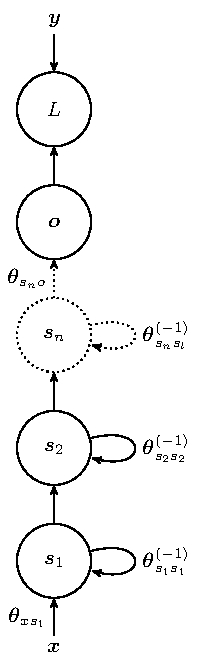
\includegraphics[]{figs/rnn.pdf}}
    \newsavebox{\rnnuf}
    \savebox{\rnnuf}{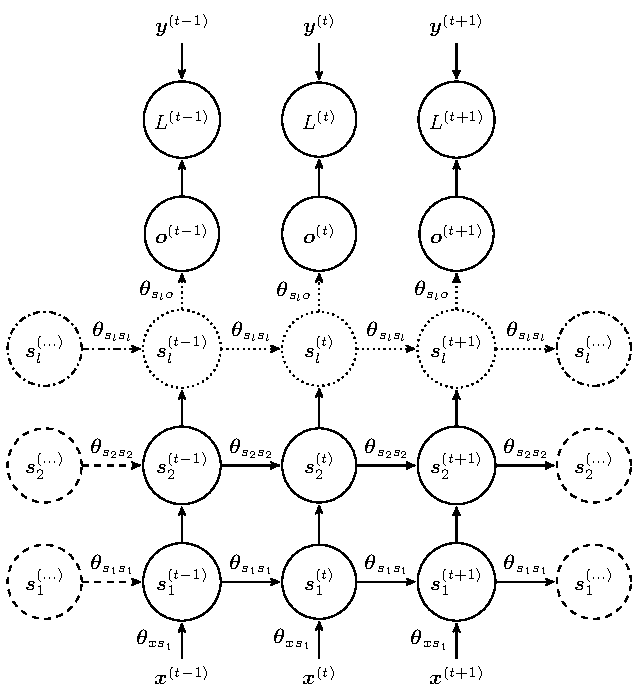
\includegraphics[]{figs/rnn_uf.pdf}}

    \begin{tabular}{p{\wd\rnn}|p{\wd\rnnuf}}
      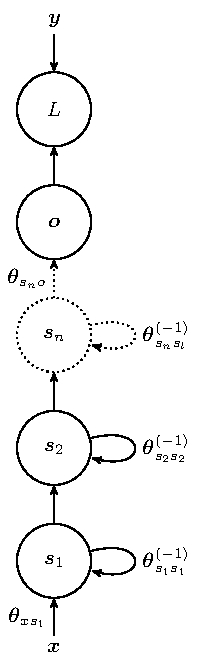
\includegraphics[width=.7\wd\rnn]{figs/rnn.pdf}  & 
                                                         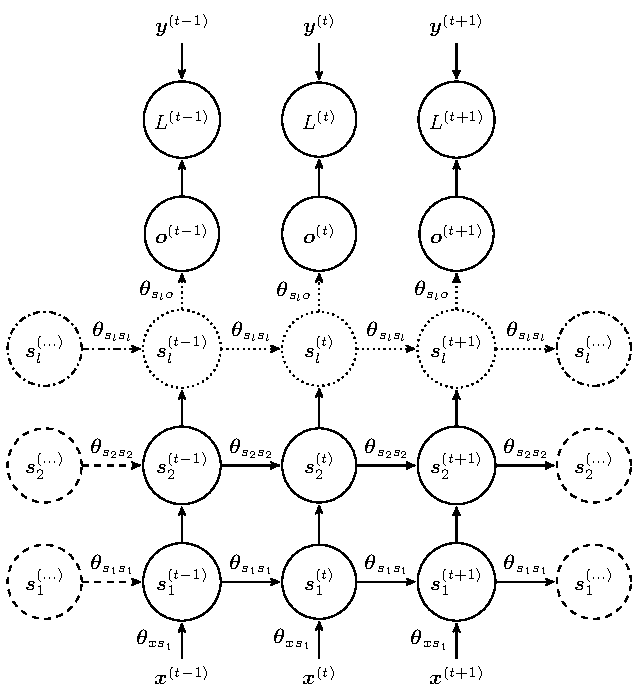
\includegraphics[width=.7\wd\rnnuf]{figs/rnn_uf.pdf}  
    \end{tabular}

  \end{frame}


  \begin{frame}{Training RNNs is difficult}
    
    \begin{equation*}
      L(\vc{o},\vc{y}) = \frac{1}{TV} \sum_t \sum_v(
      \vc{o}\tm{t}_v - \vc{y}\tm{t}_v
      )^2
    \end{equation*}

    \begin{itemize}
      \item but mini-batch SGD-flavor training still works
        \begin{equation*}
          \Delta \vc{\theta} =
          -\alpha
          \frac{1}{|M|} \sum_{(\vc{x}_m,\vc{y}_m) \in M}
          \frac{\partial{L}(
            \vc{o}%(\x_m;\vc{\theta})
            ,\vc{y}_m)}
          {\partial{\vc{\theta}}}
        \end{equation*}
      \item acute vanishing gradient problem
        \begin{equation*}
          \frac{\partial{L}\tm{t}}{\partial{\vc{W}_{ss}}} = 
          \sum_{i=0}^T
          \frac{\partial{    L}\tm{ t}}{\partial{\vc{o}\tm{t}}}
          \frac{\partial{\vc{o}}\tm{t}}{\partial{\vc{s}\tm{t}}}
          \left(
            \prod_{j=i+1}^{T}
            \frac{\partial{\vc{s}}\tm{j}}{\partial{\vc{s}\tm{j-1}}}
          \right)
          \frac{\partial{\vc{s}}\tm{i}}{\partial{\vc{W}_{ss}}}
        \end{equation*}
      \end{itemize}

    \end{frame}


    \begin{frame}{Understand vanishing gradient problem through computational graph for $T=4$}

      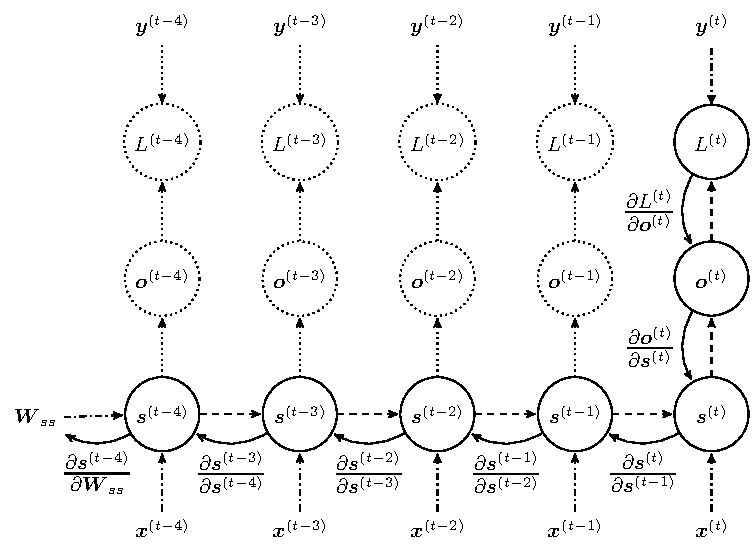
\includegraphics[width=\textwidth]{figs/grad.pdf}

    \end{frame}


    \begin{frame}{Long Short Term Memory (LSTM) `cells' store information but are more complicated than vanilla RNNs' $tanh$}

      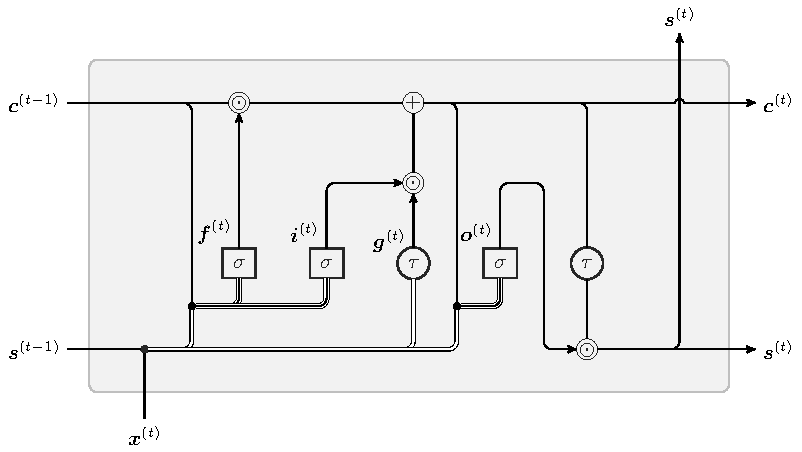
\includegraphics[width=\textwidth]{figs/lstm.pdf}
      \footcite{Colah2015}
    \end{frame}



    \section{Using RNNs for Anomaly Detection}

    \begin{frame}{Use same procedure for test time series to test generality}
      
      \begin{enumerate}
      \item sample
      \item setup RNN autoencoder
      \item train
      \item optimize
      \item evaluate anomaly scores
      \end{enumerate}

    \end{frame}


    \begin{frame}{1. Sample with sliding windows of varying length to test versatility}
      
      \begin{enumerate}
      \item spikes
      \item sine
      \item power demand
      \item electrocardiogram (ECG)
      \item polysomnography ECG (PSG-ECG)
      \end{enumerate}

    \end{frame}


    \begin{frame}{2. Setup RNN autoencoder}

      \begin{itemize}
      \item Set target to (uncorrupted) input
        \begin{equation*}\vc{y}=\vc{x}\end{equation*}
      \item Add noise to input
        \begin{equation*}
          \tilde{\x} = \x
          + \mathcal{N}(0,(0.75\sigma_{\mathrm{std}}(\x))^2)
        \end{equation*}
      \end{itemize}

    \end{frame}


    \begin{frame}{3a. Train: RMSprop is appropriate algorithm}
      
      \begin{itemize}
      \item works with mini-batch learning as data is highly redundant
      \item similar in results to second order methods with less computational cost
      \end{itemize}

    \end{frame}


    \begin{frame}{3b. Optimize RNN hyperparameters to find best RNN configuration}
      
      Optimize
      \begin{itemize}
        \item number of layers, $l$
        \item `size' of each layer, $n$
      \end{itemize}
      % could have kept size of each layer a var but kiss

      using Bayesian optimization
      \begin{itemize}
      \item minimize expensive objective function calls
      \item considers stochasticity of function
      \end{itemize}

    \end{frame}

    
    \begin{frame}{Optimization of spike-1}
      % i guess rnn is seeing val and trn as same even tough i chopped up the data into different sizes and views
      % was hoping to see l=2 lower
      % sometimes it gets stuck. hope not a false opt

      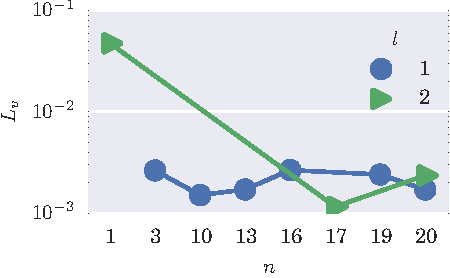
\includegraphics[width=.5\textwidth]{figs/bo_spikelv.pdf}
      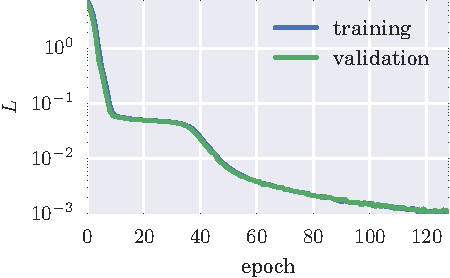
\includegraphics[width=.5\textwidth]{figs/trn_spikelv.pdf}
      
    \end{frame}


    \begin{frame}{Optimization of spike-2}

      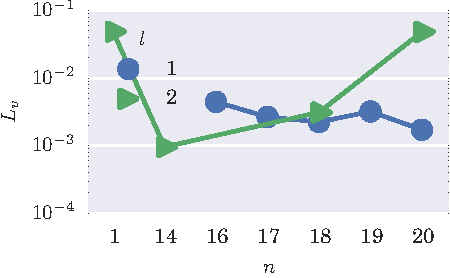
\includegraphics[width=.5\textwidth]{figs/bo_spikereg.pdf}
      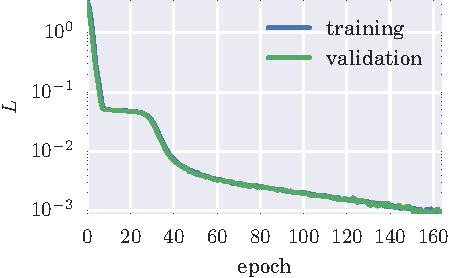
\includegraphics[width=.5\textwidth]{figs/trn_spikereg.pdf}
      
    \end{frame}


    \begin{frame}{Optimization of sine}

      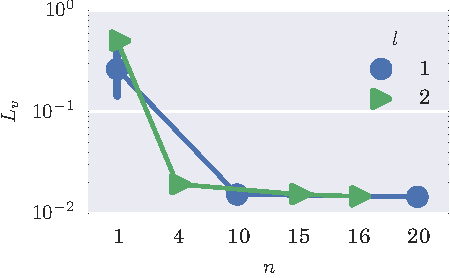
\includegraphics[width=.5\textwidth]{figs/bo_sin.pdf}
      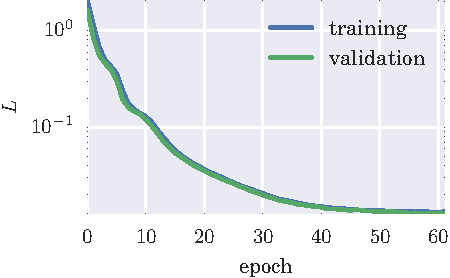
\includegraphics[width=.5\textwidth]{figs/trn_sin.pdf}
     
    \end{frame}


    \begin{frame}{Optimization of power}

      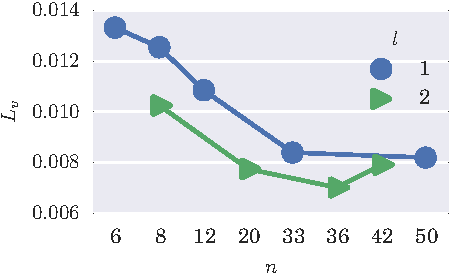
\includegraphics[width=.5\textwidth]{figs/bo_power.pdf}
      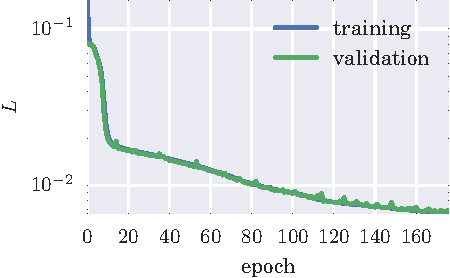
\includegraphics[width=.5\textwidth]{figs/trn_power.pdf}
      
    \end{frame}


    \begin{frame}{Optimization of ECG}

      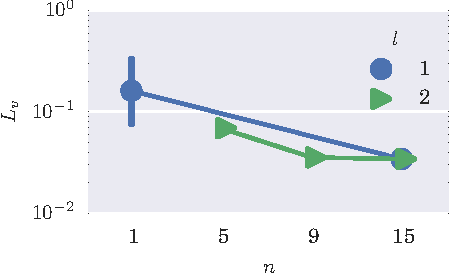
\includegraphics[width=.5\textwidth]{figs/bo_ecg.pdf}
      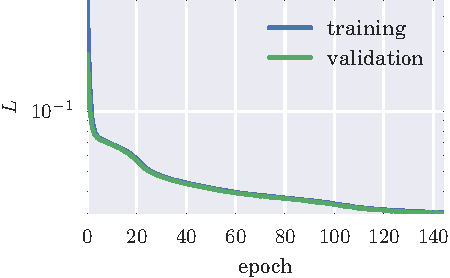
\includegraphics[width=.5\textwidth]{figs/trn_ecg.pdf}
      
    \end{frame}


    \begin{frame}{Optimization of PSG-ECG}

      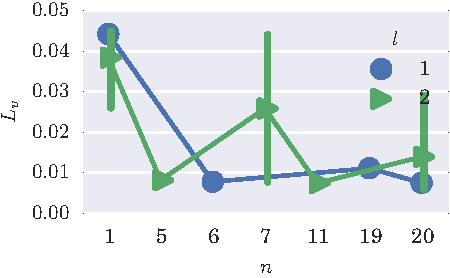
\includegraphics[width=.5\textwidth]{figs/bo_sleep.pdf}
      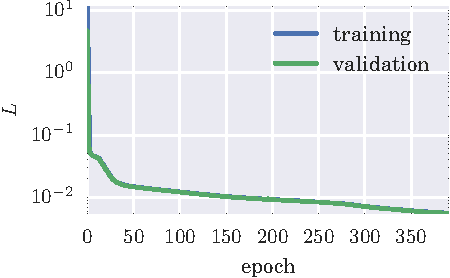
\includegraphics[width=.5\textwidth]{figs/trn_sleep.pdf}
      
    \end{frame}


    \begin{frame}{4. Use squared error as an anomaly score}

      Reconstruction Error
      \begin{itemize}
      \item individual squared error
      \item mean squared error of a window
      \end{itemize}

    \end{frame}
    

    \begin{frame}{spike-1: atypical value detected}

      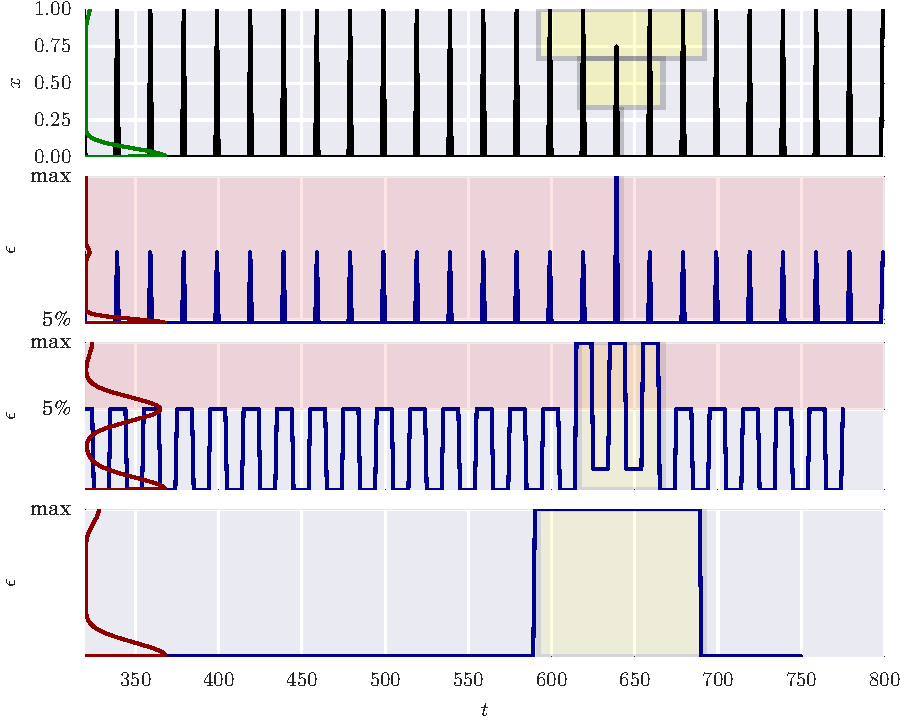
\includegraphics[width=\textwidth]{figs/er_spikelv.pdf}

      \note[item]{lower value more of a challenge}

    \end{frame}


    \begin{frame}{spike-2: irregularity detected}

      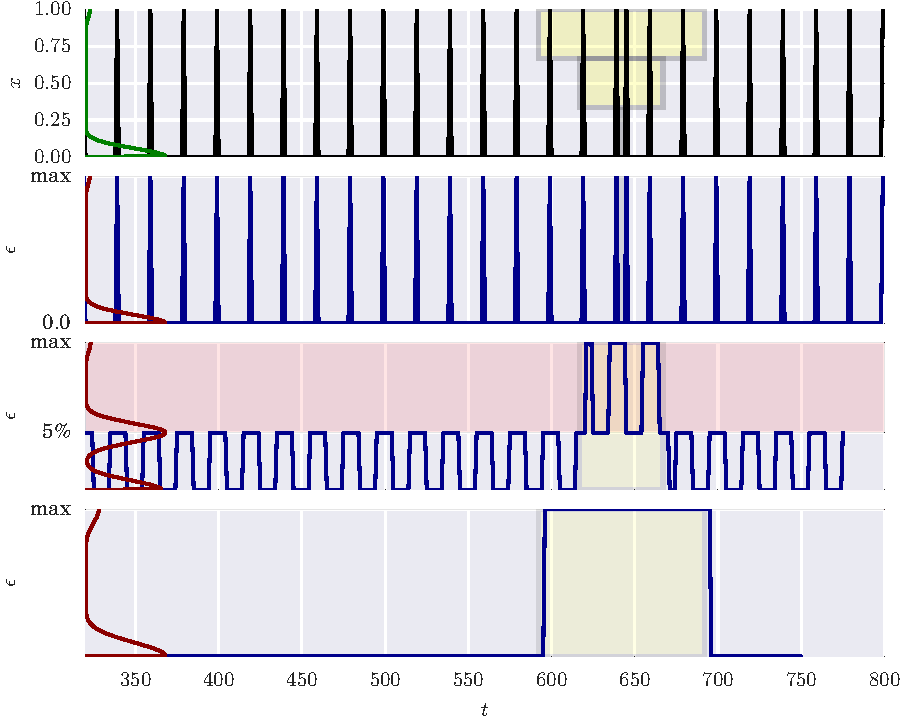
\includegraphics[width=\textwidth]{figs/er_spikereg.pdf}

    \end{frame}


    \begin{frame}{sine: discord detection inconclusive}
      %pdf not accurate
      \centering
      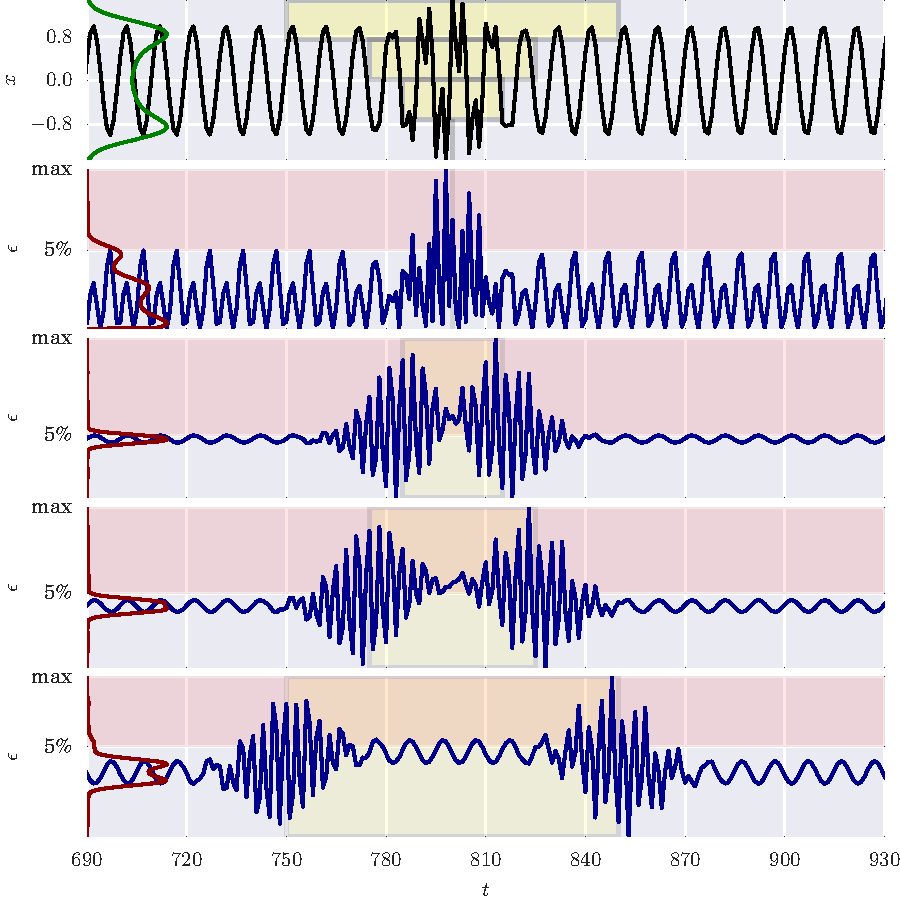
\includegraphics[height=\textheight]{figs/er_sin.pdf}

    \end{frame}


    \begin{frame}{power: discord detected}

      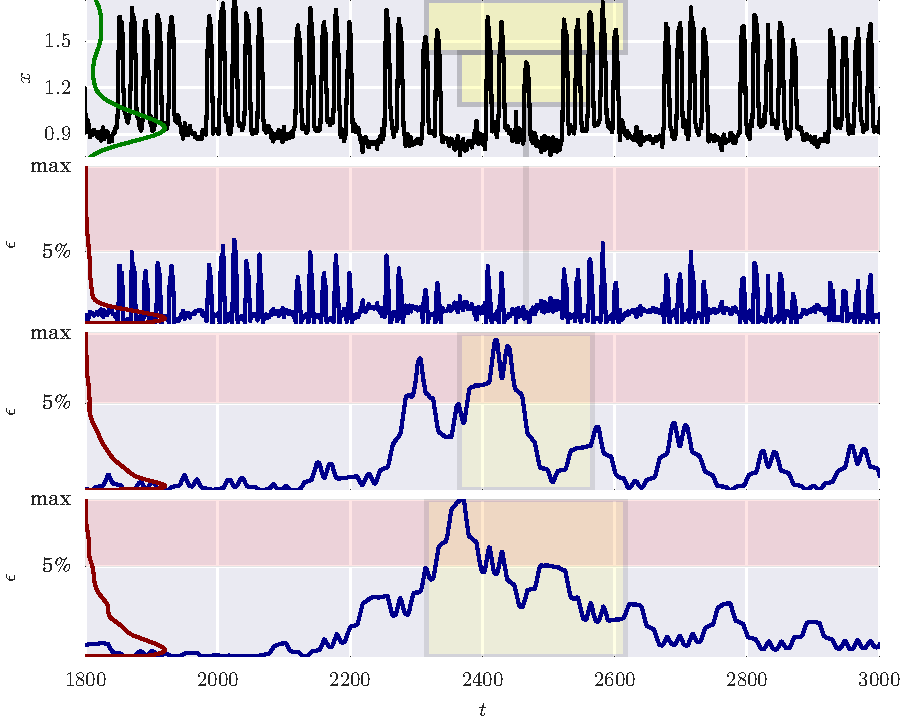
\includegraphics[width=\textwidth]{figs/er_power.pdf}

    \end{frame}


    \begin{frame}{power: discord detected}

      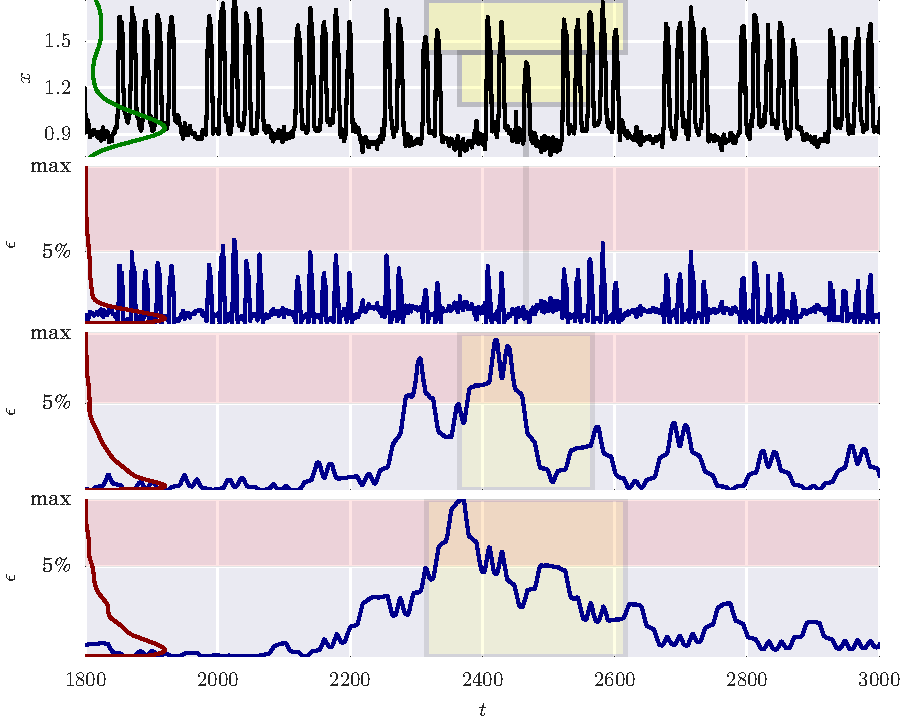
\includegraphics[width=\textwidth]{figs/er_power.pdf}

    \end{frame}


    \begin{frame}{ECG: discord detected}

      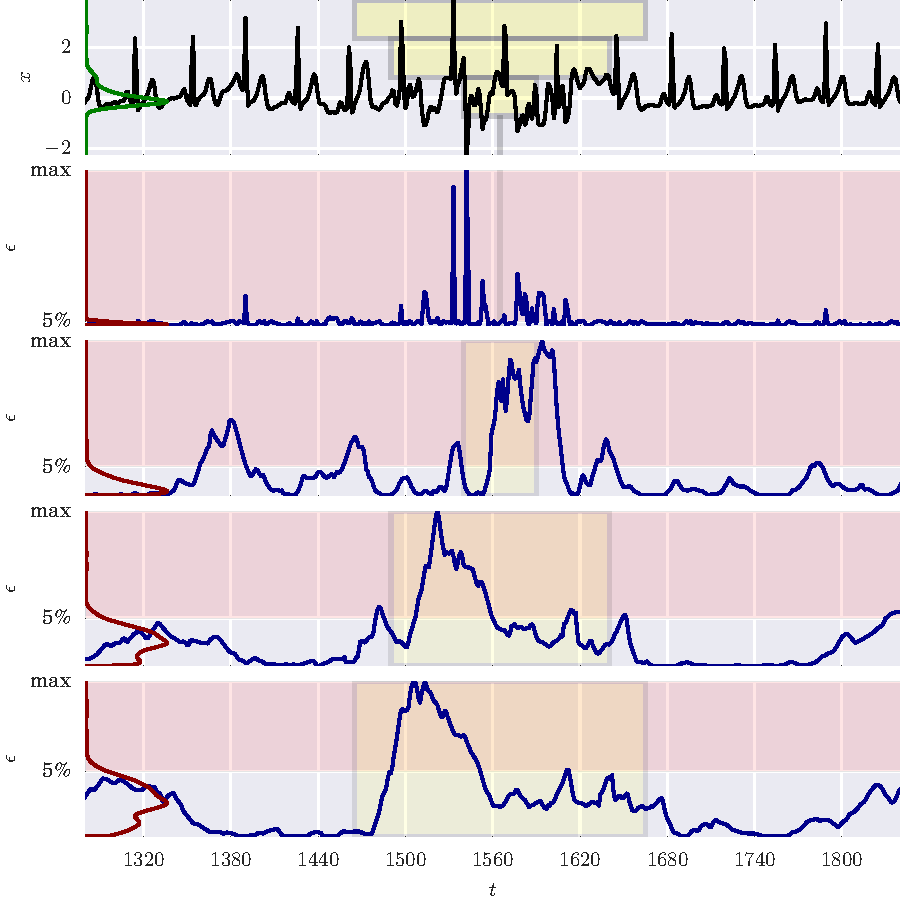
\includegraphics[height=\textheight]{figs/er_ecg.pdf}

    \end{frame}


    \begin{frame}{PSG-ECG: discord detected}

      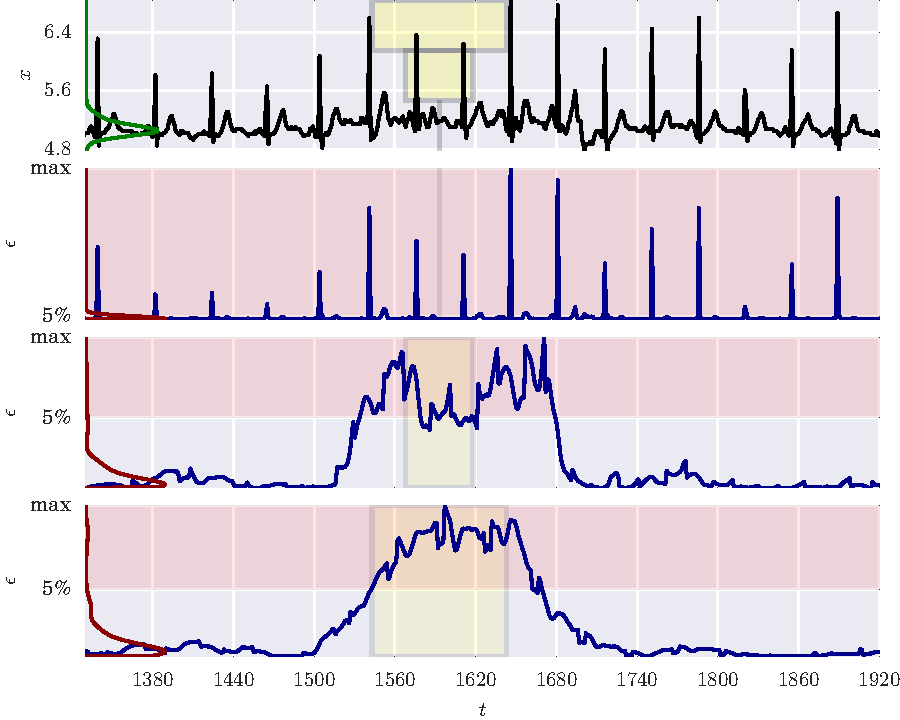
\includegraphics[width=\textwidth]{figs/er_sleep.pdf}

    \end{frame}



    \begin{frame}{Experiment conclusion: squared reconstruction error of AE-RNNs can be used to detect anomalies}

      \begin{itemize}
        \item point errors may find extreme values
        \item windowed errors find anomalies if size is on the order of anomaly
        \item RNNs were insensitive to translation and length
        \item the same process found anomalies in all tests
        \item RNNs learned normal \emph{behaviour} despite having some anomalies in the training data
      \end{itemize}

    \end{frame}


    \section{Conclusions}

    \begin{frame}{RNNs have advantages over advanced techniques}

      Model-based: HMMs
      \begin{itemize}
        \item more efficient encoding
        \item varying sequence length
      \end{itemize}

      Proximity-based: HOT SAX
      \begin{itemize}
        \item more efficient \emph{after training}
        \item multivariate
        \item not forced to find an anomaly
      \end{itemize}

    \end{frame}


    \begin{frame}{Alternative method checklist}

      \begin{itemize}
      \item Does other data need to be accessed?%
        (Is a summary of the data stored?)

      \item Is it robust against some window length?

      \item Is it invariant to translation? (Is it invariant to sliding a window?)

      \item Is it fundamentally a sequence modeler?

      \item Can it handle multivariate sequences?

      \item Can the model prediction be associated with a probability?

      \item Does it need labeled data? If not, is it robust to anomalous training data?

      \item Does it require domain knowledge?

      \end{itemize}

    \end{frame}


    \begin{frame}{Main disadvantage of RNNs: computational cost}
      \begin{itemize}
        \item training
        \item hyperoptimization
      \end{itemize}
        
    \end{frame}


    \begin{frame}{Further work is needed to strengthen the case for using RNNs for anomaly detection}
      \begin{itemize}
        \item better optimize
        \item use autocorrelation to determine minimum window length
        \item accelerate training: normalization, optimium training data size
        \item use drop out to guard against overfitting
        \item experiment with RNN architectures: bi-directional RNNs, LSTM alts., more connections
        \item incorporate uncertainty
        \item objective comparisons with labelled data
        \item try multivariate series
      \end{itemize}
        
    \end{frame}


    \begin{frame}{Conclusion}

      Use RNNs to find anomalies when computational cost can be managed.

    \end{frame}


    \section{Reproducibility}

    \begin{frame}{Technology stack enables automation and reproducibility}

      \newcolumntype{T}{!{\color{blue} \vrule width 4\arrayrulewidth}}
      \newcolumntype{C}[0]{>{\centering\let\newline\\\arraybackslash\hspace{0pt}}m{1.3in}}

      \centering 
      \begin{tabular}{l C C}
         \Xhline{6\arrayrulewidth}
         application   
         &  \multicolumn{1}{TcT}{\cellcolor{blue!10}\ldots}
        & \multicolumn{1}{TcT}{\cellcolor{blue!10}\ldots} 
        \\
        \hline
        container network 
        & \multicolumn{2}{TcT}{\cellcolor{blue!10}\textsf{Weave}}  
        \\
        app. containerization  
        & \multicolumn{2}{TcT}{\cellcolor{blue!10}\textsf{Docker}}   
        \\
        \hline
        operating system 
        & \multicolumn{2}{TcT}{\cellcolor{blue!10}\textsf{CoreOS}} 
        \\ 
        \hline
        machine 
        & \multicolumn{1}{TcT}{\cellcolor{blue!10}(x64)}
        &  \multicolumn{1}{TcT}{\cellcolor{blue!10}x64} 
        \\ 
        \hline
        hypervisor 
        & \multicolumn{1}{TcT}{\cellcolor{blue!10}\textsf{VirtualBox}} 
        & \multicolumn{1}{TcT}{\cellcolor{blue!10}\ldots }
        \\
        hypervisor interface
        & \multicolumn{1}{TcT}{\cellcolor{blue!10}\textsf{Vagrant}} 
        & \multicolumn{1}{TcT}{\cellcolor{blue!10}\textsf{AWS}}
        \\
        \hline
        host operating sys. 
        & \multicolumn{1}{|c|}{
          \textsf{Windows}%
          \textbar \textsf{OS X}%
          \textbar \textsf{Linux}
          }
        & \multicolumn{1}{TcT}{\cellcolor{blue!10}\ldots}
        \\
        \hline
        hardware 
        & \multicolumn{1}{|c|}{x64}
        & \multicolumn{1}{TcT}{\cellcolor{blue!10}x64}
        \\
        \Xhline{6\arrayrulewidth}
        & local 
        & remote
      \end{tabular}

    \end{frame}


    \begin{frame}{Reproducibility of technology stack on any machine enables parallel processing}
        \includegraphics[width=\textwidth]{appendix/figs/arch.pdf}
    \end{frame}

    \section{Discussion Time}

% endp

%  \begin{frame}[allowframebreaks]{References}
%    %
%  \end{frame}

% /other/ contribs

\end{document}

